\chapter{Introduction}
\label{ch:intro}
\hl{Intro to the first chapter
Give a nice history of solar observations and discuss current observing efforts as well as modeling efforts, but briefly; quickly move into atmosphere, corona}
\par The Sun is the most important celestial body to life on Earth. For the last five billion years, it has provided the light by which humans observe the world around them and the heat to save the planet from the frigid temperatures of interplanetary space. Because of its proximity, the Sun provides astronomers an exclusive and unique look into how stars behave. By observing and understanding the Sun, one can make conclusions about other types of stars in our galaxy and the universe.
%
\par Perhaps no other consistent celestial event has attracted as much attention as the solar eclipse. Solar eclipses have been observed and recorded for thousands of years, with some reports dating back to the fourteenth century BC \citep{golub_solar_2010}. The recordings of ancient eclipses have been heavily studied. Chinese rock drawings dating back to the Han dynasty (approximately 1900 years ago) appear to show the moon completely obscuring the Sun. Additionally, some have even suggested the Aubrey holes that surround the Stonehenge site were used to track and predict both solar and lunar eclipses \citep{golub_solar_2010}. Though some claims of ancient eclipse studies are controversial, it suffices to say that humans have long sought to study and explain the behavior of the nearest star to Earth.
%
\begin{figure}
	\centering
	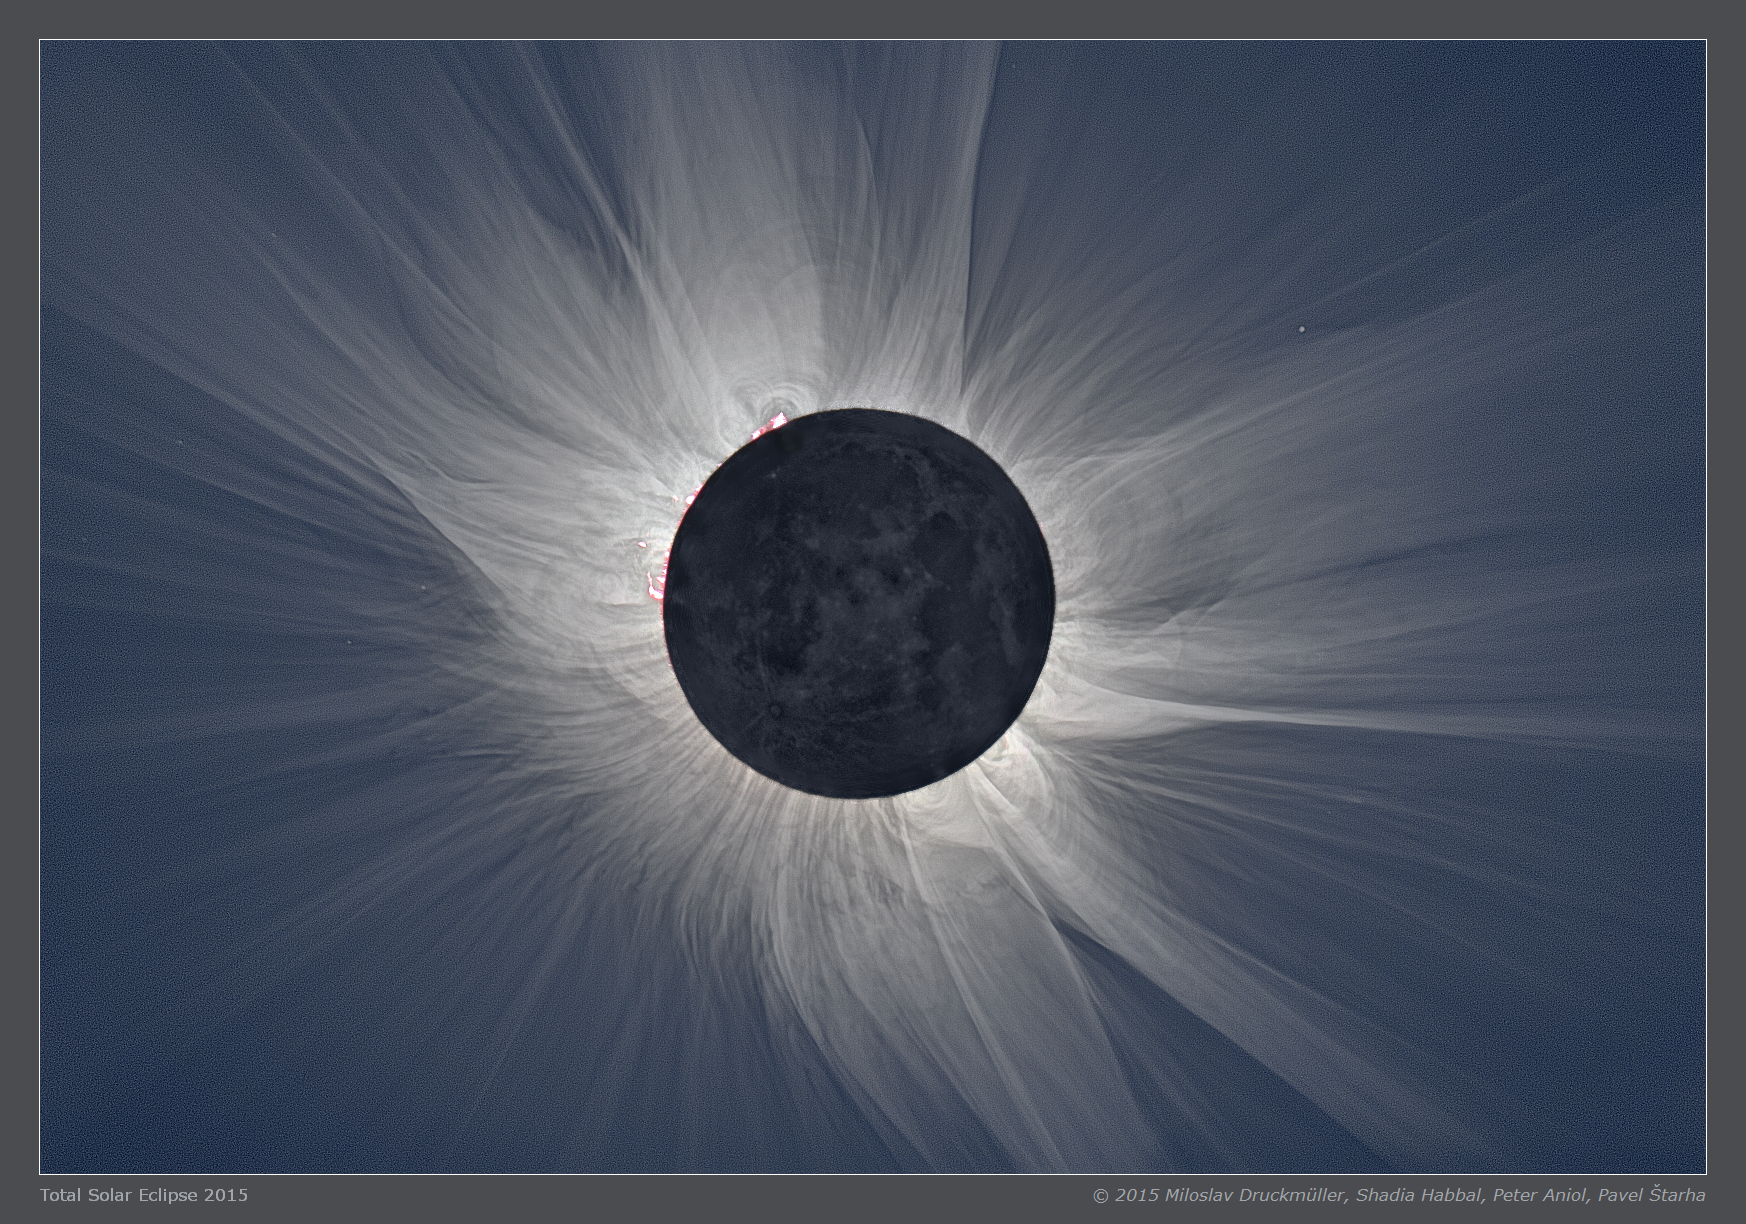
\includegraphics[width=0.7\textwidth]{figures/Tse_2015_Svalbard_800mm_Nikon_D810.png}
	\caption{Total eclipse as seen from Svalbard, Norway on March 20, 2015. Open and closed loops in the highly-structured solar corona are clearly visible. Photo courtesy of Miloslav Druckm\"{u}ller.}
	\label{fig:solar_eclipse}
\end{figure}
%
\par In particular, solar eclipses have captured the attention of artists for centuries. Cosmas Damian Asam, a Bavarian painter and architect active in the early eighteenth century, used images of solar eclipses in many of his works, including several frescoes and an altarpiece. \citet{olson_st._2007} discuss how Asam, a deeply religious artist, was commissioned several times to depict the vision of St. Gregory the Great, a Benedictine monk, as described in his work \textit{Dialogues}. 
%
\par One of these depictions, an altarpiece at a Benedictine monastery in Kladruby, Czech Republic (see Fig. 7 of \citet{olson_st._2007}), shows ``the visionary globe surrounded by a glowing halo of yellow light that more closely resembles the solar corona'' \citep{olson_st._2007}. An additional altarpiece at another monastery in Weltenburg, Germany shows a perhaps even more pronounced depiction of the solar corona during a total solar eclipse. \citet{olson_st._2007} note that, given his detailed depictions, Asam must have observed several solar eclipses as well as the solar corona, with these astronomical events profoundly impacting his depictions of supernatural events in his works. This is but one example of how solar eclipses and their consequential insight into the highly structured solar atmosphere, have shaped scientific and artistic discourse througout history.
%
%%
\section{Structure of the Solar Atmosphere}
\label{sec:structure}
\hl{This section will discuss the structure of the solar atmosphere including the different layers of the Sun and how they are connected. This will help to introduce the solar corona}
\par Though the Sun can be easily seen from Earth, its dynamic and highly structured atmosphere is not observable with the naked eye, with the one exception being brief glimpses of the corona during an eclipse. The interior of the Sun is of course very complex and constitutes a very different regime of physics than that seen in the solar atmosphere. Thus, this work will be primarily limited to the upper solar atmosphere with some discussion of the lower layers.
%
\par The solar atmosphere is often divided up into four separate regions: the photosphere, the chromosphere, the transition region, and the corona. Fig. \ref{fig:cartoon_layers} shows a cartoon of the different layers while Fig. \ref{fig:graph_layers} shows the density and temperature profiles of the atmosphere with each region labeled. The \textit{photosphere} is what we typically refer to as the solar surface, with the actual surface located where the optical depth, $\tau$, is equal to 1. This region also contains the lowest temperature on the Sun, approximately 4400 K, located about 525 km above the surface \citep{carroll_introduction_2007}. The photosphere is where the majority of the visibly (with the naked eye) observable photons originate.
%
\par The temperature minimum defines the top of the photosphere above which lies the \textit{chromosphere}. As can be seen from Fig. \ref{fig:graph_layers}, the density in the chromosphere is many orders of magnitude less than that of the photosphere and the temperature has increased from the minimum up to about $1\times10^4$ K. Though not visible with the naked eye, the chromosphere is highly structured. Structures such as spicules, tall columns of gas that extend high into the solar atmosphere thought to heavily impact the behavior of plasma in the corona \citep{de_pontieu_origins_2011}, originate in the photosphere as well as filaments, essentially spicules observed on-disk and plage, bright regions surrounding sunspots.
%
\begin{figure}
	\centering
	\subfigure[]{%
	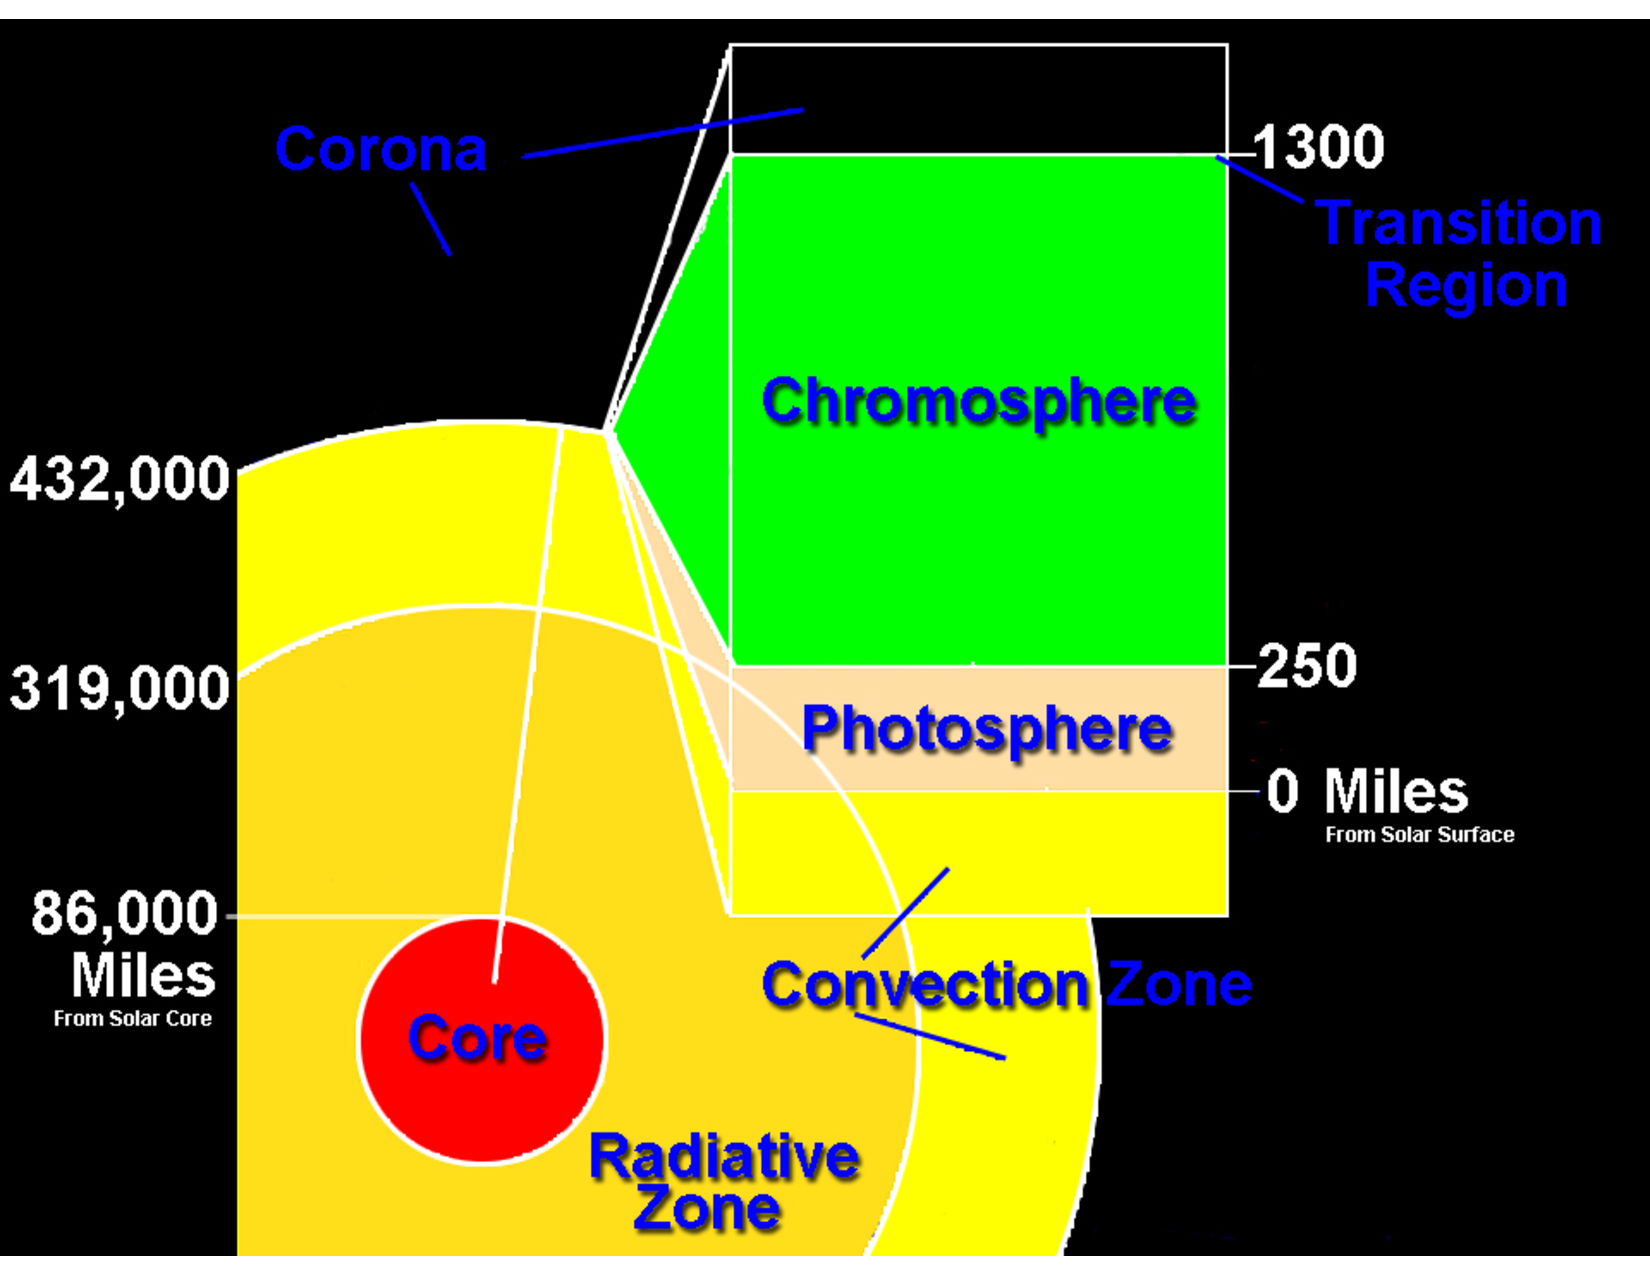
\includegraphics[width=0.45\textwidth]{figures/cartoon_layers.pdf}
	\label{fig:cartoon_layers}}
	\subfigure[]{%
	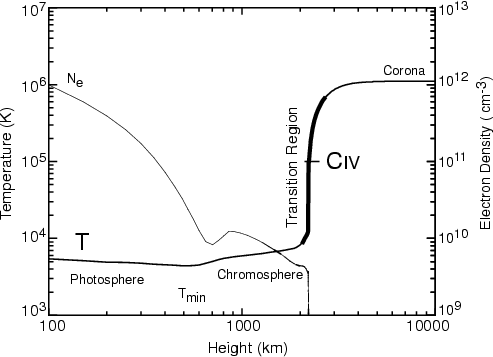
\includegraphics[width=0.45\textwidth]{figures/diagram_layers.png}
	\label{fig:graph_layers}}
	\caption{Layers of the solar atmosphere \textbf{(a)}Courtesy of NASA \textbf{(b)} Taken from \citet{gary_solar_2007}}
	\label{fig:layers}
\end{figure} 
%
\par Next is the \textit{transition region}, so called because of the steep temperature and density gradients (see Fig. \ref{fig:graph_layers}) that mark the transition between the chromosphere and the corona. The transition region is extremely thin, only a few hundred kilometers as compared to the chromosphere which extends over many thousands of kilometers. However, in this very short change in altitude, the temperature in the solar atmosphere jumps from $\approx1\times10^4$ K to temperatures exceeding $1\times10^5$ K. 
%
\par Finally, the solar \textit{corona}, or ``crown'', is the highly-dynamic uppermost layer of the Sun's atmosphere. Visible with the naked eye only during a total solar eclipse (see Fig. \ref{fig:solar_eclipse}), the corona is highly-structured and diffuse. Here, the temperature continues to increase, with typical coronal temperatures exceeding $1\times10^6$ K. Particularly high temperatures ($\approx1\times10^7$ K) have also been observed in \textit{active regions}, sites of intense magnetic activity associated with sunspots. These active regions can contain plasma as cool as $1\times10^4$ K as well and represent some of the most dynamic portions of the solar corona.
%
\par The work presented here will focus primarily on the plasma dynamics in the corona, in particular, in the cores of active regions where the intense magnetic field drives the motion of the plasma. In the following sections, we will discuss the origin of the solar magnetic field, its topology, how it impacts plasma in the solar corona, and finally how it connects to the anomalously high temperatures seen in the upper solar atmosphere.
%%
\section{The Solar Magnetic Field}
\label{sec:magnetic_field}
\hl{touch on field origin (dynamo theory), discuss how the field gets tangled, formation of loops, drives behavior of the atmosphere, lead into discussion of coronal heating, low beta versus high beta}
%
\par Because of the high temperatures that characterize both the solar atmosphere and interior, much of the gas that makes up the Sun is ionized; that is, each atom has been stripped of at least one of its electrons. This means that the Sun is filled by a sea of charged particles, or plasma. In the corona where temperatures are often higher than $1\times10^6$ K, even heavy elements such as Mg, Ca, and Fe are stripped of their electrons. Because these particles are charged, their motion is strongly dictated by both the electric and magnetic fields via the Lorentz force law. Thus, to understand the dynamics of the coronal plasma, one must first try to understand the magnetic field that ultimately controls it.
%
\par The Sun, like the Earth, possesses an intrinsic magnetic field, though its origin and dynamics constitute a largely unsolved problem. Additionally, unlike Earth, the solar magnetic field is highly dynamic and comparatively quite strong (up to 1000 G in sunspots as compared to the $<1$ G field on Earth) \citep{aschwanden_physics_2006}. From the earliest studies of magnetism, it has been known that a conductor moving through a magnetic field produces a current. This current then in turn produces an additional magnetic field. Treating the convection zone (below the photosphere) plasma as the conductor and assuming some preexisting, but small magnetic field leads to what is commonly known as \textit{dynamo theory} \citep{golub_solar_2010}.
%
\begin{figure}
	\centering
	\subfigure[]{%
	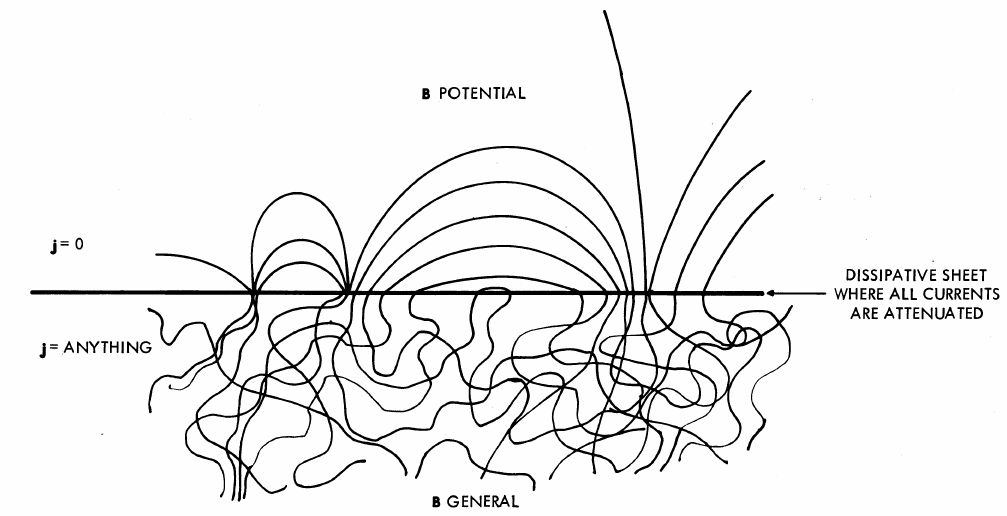
\includegraphics[width=0.45\textwidth]{figures/piddington_cartoon.png}
	\label{fig:cartoon_flux}}
	\subfigure[]{%
	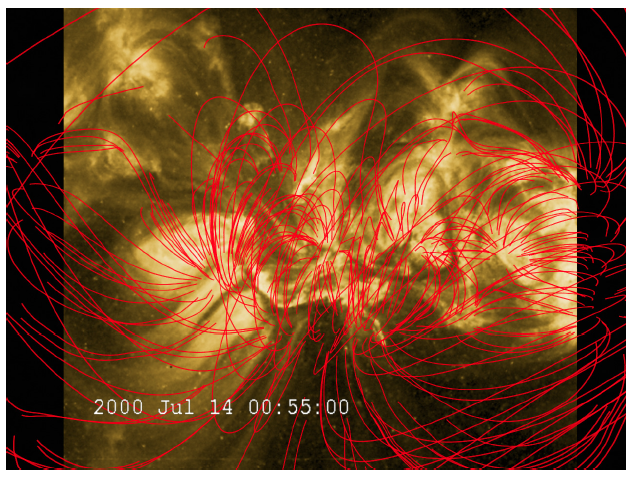
\includegraphics[width=0.45\textwidth]{figures/mag_field_extrapolation.png}
	\label{fig:mag_extrap}}
	\caption{\textbf{(a)} Flux emergence from twisted and tangled field below the photosphere yields loop structures that stretch high into the solar atmosphere. Taken from \citet{gold_magnetic_1964}.\textbf{(b)} The coronal magnetic field topology is extremely complex, making determinations of coronal plasma dynamics difficult. Shown here is a magnetic field extrapolation constructed from an optical magnetogram. An image from the TRACE satellite is superimposed to show the loop structures. Taken from \citet{reale_coronal_2010}.}
	\label{fig:complex_fields}
\end{figure}
%
\par Dynamo theory seeks to show self-consistently how the interaction between the Sun's hot plasma and some small initial field leads to the observed complicated topologies and field strengths. Modeling such a system is no easy task as the interactions between the field and the plasma are highly non-linear, meaning solving the so-called ``dynamo equations'' requires a significant amount of computational effort. But how does this field affect the plasma dynamics of the corona? The solar magnetic field is said to be \textit{frozen in} to the solar plasma; that is, the field moves with the plasma. Since the Sun is not solid, it undergoes \textit{differential rotation}, meaning that different latitudes are spinning at different rates. Since the field follows the motion of the plasma, this causes the normally dipolar (north-south aligned) field to have an east-west component. This amplified and twisted field is then carried up to the photosphere by magnetic buoyancy, an idea first proposed by \citep{parker_formation_1955}, resulting in dipolar loop-like structures poking through the solar atmosphere (see Fig. \ref{fig:cartoon_flux}). This phenomenon, commonly referred to as magnetic flux emergence, is by no means a solved problem and is a continuing topic of research \citep[see][]{cheung_flux_2014}. Finding out how the solar magnetic field is generated and how it makes its way to the upper atmosphere will undoubtedly help to explain much of the observed plasma dynamics in the corona.
%
\begin{figure}
	\centering
	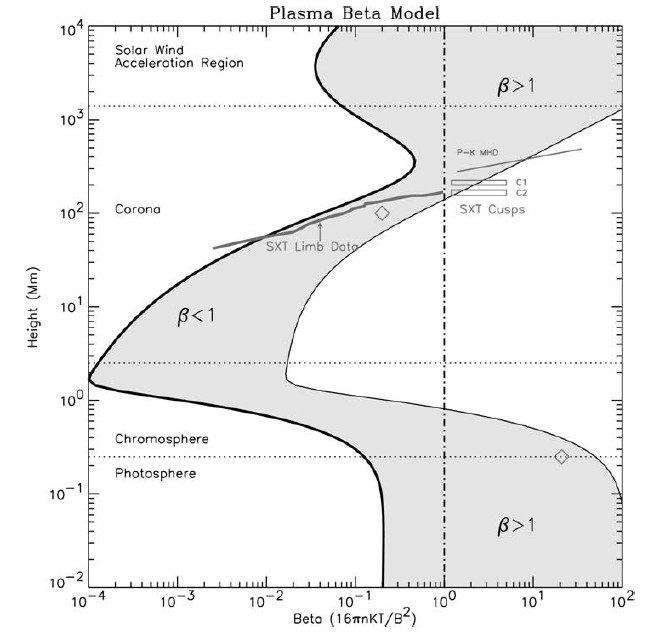
\includegraphics[width=0.6\textwidth]{figures/plasma_beta.png}
	\caption{Taken from \citet{gary_plasma_2001}.}
	\label{fig:plasma_beta}
\end{figure}
%
\par Fortunately, we can still learn something about the corona without completely solving the problem of where the driving magnetic field comes from. The corona constitues what is commonly referred to as a ``low-beta plasma'' such that $\beta=p_{\mathrm{thermal}}/(B^28\pi)$, the ratio between the gas pressure and magnetic pressure, is $\beta<1$ (see Fig. \ref{fig:plasma_beta}). This means that coronal magnetic field acts as a guide for the plasma, with the flow directed primarily in the field direction with negligible cross-field motion. A useful analogy is that of water flowing through a pipe: the rigid pipe directs the flow of the water, but has no affect on the underlying fluid dynamics. Provided the field is reasonably stable and the relevant fluid equations are parameterized in terms of the field-aligned coordinate, our equations governing the plasma dynamics need not include the field at all!
%
\par \hl{Talk about drawbacks, mention MHD and hydrodynamic and hydrostatic; lead into coronal heating conversation; not sure if this is actually needed here...}
%%
\section{The Coronal Heating Problem}
\label{sec:heating}
\hl{Here discuss coronal heating broadly, first evidence for high coronal temperatures, some proposed heating mechanisms, magnetic reconnection, AC versus DC heating, wave heating versus braiding etc. Use Klimchuk review of coronal heating for this section + Cargill nanoflare paper(s)
}
%
\par Thus, far we have not addressed the important question of why the solar corona is so much hotter than the surface. From an intuitive, thermodynamic perspective, we would expect the atmospheric temperature to decrease as we moved away from the surface. However, nearly 70 years of observations have shown this is not the case and these anomalously high temperatures, dubbed the ``coronal heating problem,'' continue to baffle solar physicists today.
%
\par The discovery of the $>1\times10^6$ K corona was made over the course of nearly fifty years through many laborious spectroscopic observations. Spectroscopic measurements during the late-nineteenth and early twentieth centuries of solar eclipses and images obtained from coronagraphs yielded a suprising result:
\section{Summary}
\label{sec:summary}
%
End with outline of the rest of the thesis: in ch. such and such we will discuss such and such